% Dokumenteinstellungen
% ======================================================================

% Die Dokumentklasse definiert die Art des Dokuments
% und seine Grundeigenschaften
\documentclass[11pt,a4paper]{scrartcl}		% [Schriftgröße 10, Textbereich Din A4] {Dokumentart Artikel}


% Zusätzliche (aber sinnvolle) Pakete laden
% ======================================================================
% Pekete fügen verschiedene Funktionen zu LaTeX hinzu.
% ganz ohne Pakete wäre Latex gerade mal etwas besser als notepad...
\usepackage[a4paper]{geometry}				% DIN-A4 Größe des Papiers; sollte mit der Ausdehnung des Textes in documetnclass übereinstimmen.
\usepackage[utf8]{inputenc}					% Zeichenkodierung UTF-8 falls Probleme wegen utf8 auftreten, utf8 durch utf8x ersetzen
\usepackage[T1]{fontenc}
\usepackage{lmodern}
\usepackage{amsmath}						% erlaubt mathematische Formeln
\usepackage[english]{babel}					% Deutsche Sprache und Silbentrennung
\usepackage{amssymb}						% Verschiedene Symbole
\usepackage{graphicx}						% Zum Bilder einfügen benötigt
\usepackage{hyperref}						% Sprunglinks für Überschriften, Fußnoten und Weblinks

%Eigenes

\usepackage{subfig}							% Subfloat Benutzung, Unterteilung für Bilder

\usepackage[numbers,square]{natbib}
\bibliographystyle{alphadin}%plaindin}%unsrt}%alphadin}

\usepackage{setspace}
\usepackage{geometry}
\geometry{a4paper,left=2.5cm,right=2.5cm}

\usepackage{siunitx}
\usepackage{booktabs}
\usepackage{eurosym}

\usepackage[shortlabels]{enumitem}

\usepackage{fixltx2e}  % Für \textsubscript{}

\usepackage{tabularx}
\newcolumntype{L}[1]{>{\raggedright\arraybackslash}p{#1}}
\newcolumntype{R}[1]{>{\raggedleft\arraybackslash}p{#1}}
\newcolumntype{C}[1]{>{\centering\arraybackslash}p{#1}}

\usepackage{longtable}

\usepackage{pdfpages}

\usepackage{pstricks}	% Erstellung von Plots
\usepackage{pst-plot}



% Dokumentbeginn
% ======================================================================
% Ab hier beginnt das eigentliche Dokument.
% Alles was danach folgt wird im fertigen PDF angezeigt.

\begin{document}


% Titelblatt
% ===========================================

\begin{titlepage}
	
	\singlespacing
	\begin{center}
	
		\quad
		\vspace{1cm}
	
		\Large{\textbf{Project Work\\Cyber-Physical Systems}}
	
		\vspace{1.5cm}
	
		\huge{\textbf{Autonomous Aerobatics on\\Commanded Paths}}
	
		\vspace{1.5cm}
	
		written by
		
		\vspace{1.5cm}
	
		\Large{\textbf{Youlin Gao\\Anthony Blanc\\Andreas Bruckmeier}}
	
		\vfill
		
		submitted at the\\
		Institute for Real-Time Computer Systems\\
		Technische Universität München,\\
		to\\
		Prof. Marco Caccamo

		\vspace{1cm}		
		
		Date: 26th February 2016
	
	\end{center}
	
\end{titlepage}

\setstretch{1.2}


% Inhaltsverzeichnis   (Überschriften werden automatisch in das Inhaltsverzeichnis aufgenommen.)
% ===========================================
\newpage
\tableofcontents	

\vfill

% Abbildungsverzeichnis
% ===========================================

%\renewcommand{\listfigurename}{}
\listoffigures
%{\def\section*#1{}\listoffigures}


% Textbeginn
% ================================================================================
% ================================================================================


% Neue Seite
% ===========================================
\newpage
	

\section{Overview}

As a part of the CPS course in WS15/16, a controller structure for an aircraft in an simulation environment was built, performing autonomous aerobatics on commanded paths.
In this report, the controller structure is explained and achievements are presented.
Before, an overview of the features are given and the underlying work is clarified.

\medskip

\subsection{Working Principle and Features}

Control target of the controller is a path in 3-dimensional space as a function of time.
The controller's aim is to fly along this commanded path by determining the deviation from the given trajectory and thereout calculating acceleration commands which are the inputs of the actuator-controllers of the aircraft.

\textbf{Figure~\ref{fig_complete_structure}} depicts the complete control structure of the aerobatic controller. 
With the position data of the trajectory and actual position signals of the aircraft, the desired acceleration is computed, and by considering the gravity handed to the control structure where the acceleration in body frame is used as the control variable for the aileron-, elevator-, and rudder-control.
Also, with the position data, the delay of the aircraft from the desired path is determined and by considering a look ahead distance, the throttle is controlled with this information.

The resulting steering signals computed by the control structure are handed to the simulation environment which hands back measurement results of the virtual aircraft's sensors.
These signals are processed and provided to the control structure. A feature of the signal processing is the estimation of the aircraft-position with accelerometers and gyrometers when there is no available GPS-signal.

\begin{figure}[!h]
  \begin{center}
  	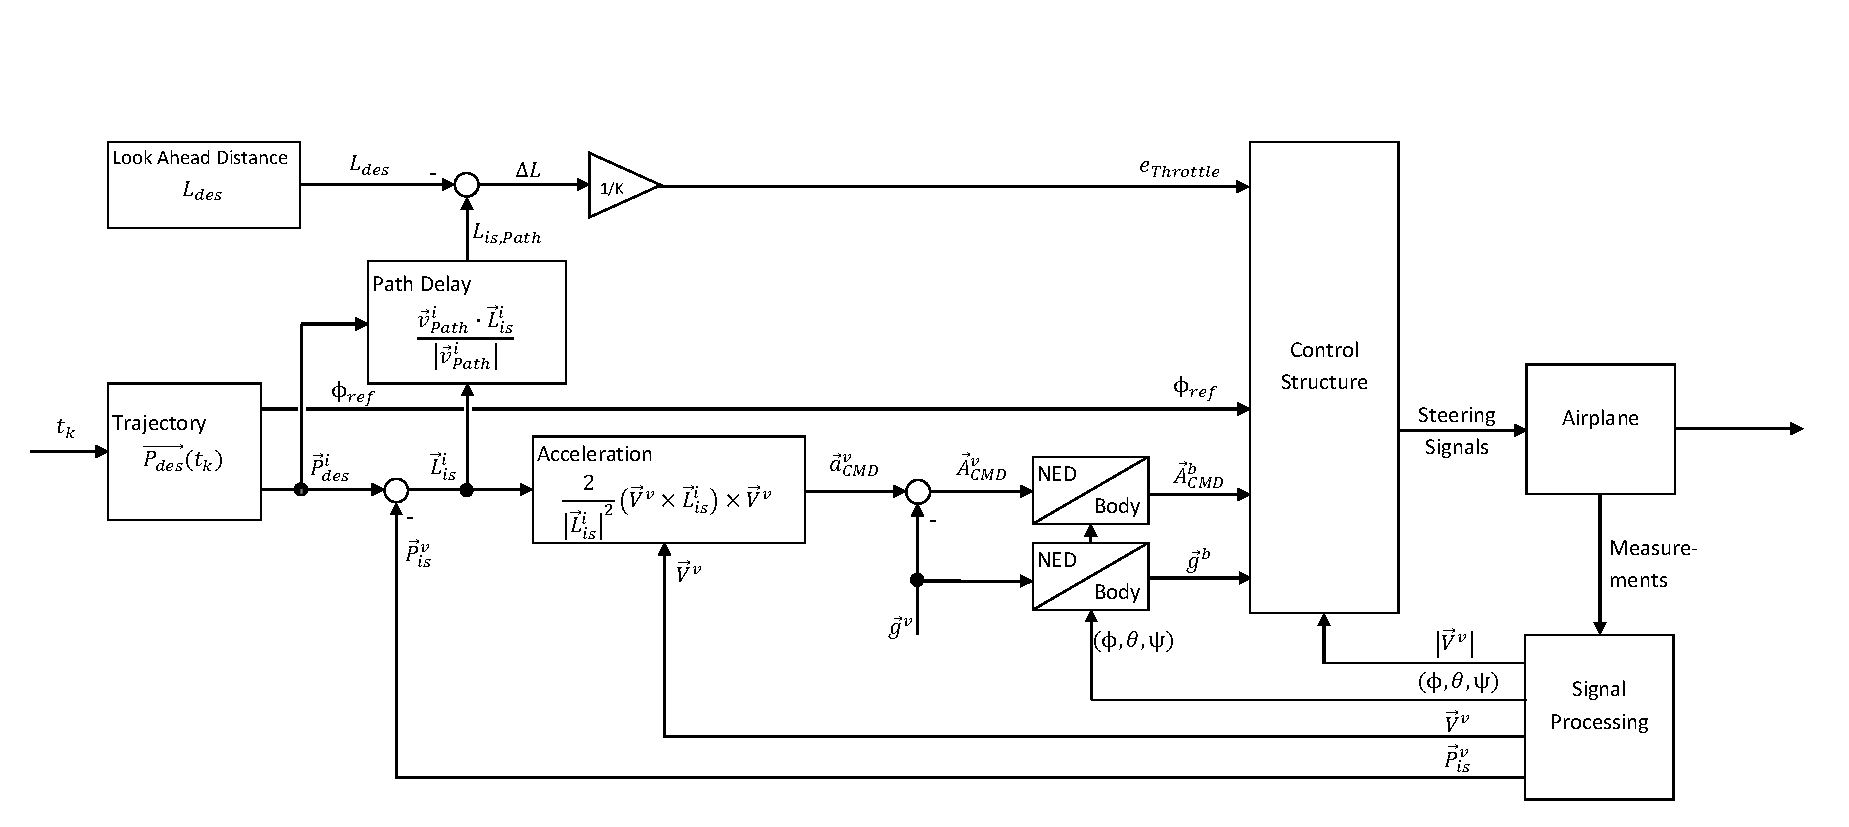
\includegraphics[width=\textheight, angle=90]{pictures/complete_structure.pdf}
  \end{center}
  \caption{Overview of the control structure of the aerobatic controller.}
  \label{fig_complete_structure}
\end{figure}


\subsection{Underlying Work}

The control structure, implemented and presented in this project work, is based on the work of Sanghyuk Park\cite{Park.2012} and modified by establishing the desired path depending on time and determining the path delay in order to control the throttle.

The estimation of the aircraft's position signal is implemented after a method which is, at the time of handing in this report, not yet published. We got the access ahead to the release by our tutor.

\section{Details}

In the following, each part of the control structure (compare Figure~\ref{fig_complete_structure}) is presented in detail.

\subsection{Interface with the Simulation Environment}

\subsection{User Interface}

\subsection{Path Generation}

\subsection{Processing of Control Variables}

\subsection{Control Structure}

\subsection{GPS Signal Estimation}

\section{Results}






% Textende
%----------------------------------------------------------------
%----------------------------------------------------------------
% Anhang

\newpage

\begin{appendix}
%\renewcommand{\refname}{A}
\section{Appendix}

\bigskip



% Literatur
% ===========================================
\subsection{References}

\begin{flushleft}
\renewcommand{\refname}{}
\singlespacing
%\bibliography{references}
{\def\section*#1{}\bibliography{references}}
\end{flushleft}

%\newpage


\bigskip

\subsection{'Variables Declaration'}

\begin{tabbing}
	 \hspace{2cm} \= \hspace{2cm} \= \hspace{3cm} \kill
	\> $t_k$ \> Point in time (time-discrete)\\	
	\> $\phi_{ref}$ \> Angle of reference vector for aileron control, forces the roll-angle\\
	\> $\vec{P}_{des}^i$ \> Desired position of the aircraft (inertial frame)\\
	\> $\vec{P}_{is}^i$ \> Actual position of the aircraft (inertial frame)\\
	\> $\vec{L}_{is}^i$ \> Difference between desired and actual position (inertial frame)\\
	\> $\vec{a}_{CMD}^v$ \> Desired Acceleration of the aircraft (vehicle frame)\\
	\> $\vec{g}^{v,b}$ \> Acceleration by gravity (vehicle,body frame)\\
	\> $\vec{A}_{CMD}^{v,b}$ \> Desired Acceleration with gravity considered (vehicle,body frame)\\
	\> $L_{des}$ \> Look ahead distance \\
	\> $L_{is,Path}$ \> Distance concerning the desired path, the aircraft lags behind \\
	\> $\Delta L$ \> Desired distance the aircraft needs to catch up \\
	\> $e_{Throttle}$ \> Input error for the throttle controller \\
	\> $(\phi,\theta,\psi)$ \> Euler angles of the aircraft \\
	\> $\vec{V}^v$ \> Velocity vector of the aircraft (vehicle frame)\\	
	
\end{tabbing}


\end{appendix}

\end{document}


% -------------------Bausteine--------------------------------------
	
%\begin{figure}[!b]
%  \begin{center}
%    \includegraphics[width=16cm]{../Machine-Epsilon-different-divisors.eps}
%  \end{center}
%  \caption{\small Figure caption. To get a figure to span two
%      columns, use the environment figure* rather than figure.}
%  \label{fig-label}
%\end{figure}


%\begin{enumerate}[{(\arabic{enumi})}]
%
%	\item
%			
%\end{enumerate}

%\begin{pspicture}[xAxisLabel=Auslastung,yAxisLabel=Herst.-Kosten](-0.5,0)(0.5,6.5)
%\begin{psgraph}[arrows=->,Dx=1,Dy=2](0,0)(-0.1,-0.1)(1.2,1.2){5cm}{4cm}
%	\psplot[plotpoints=200,linecolor=red]{0.075}{1}{0.2 0.1 x add div}
%\end{psgraph}
%\end{pspicture}

%\begin{figure}[ph]
%	\centering
%	\caption{Function with three different solvers for task~2.}
%	\lstinputlisting{../Solver.m}
%	\label{Code-Solver}
%\end{figure}

	
%\section{Literature}
%
%\renewcommand{\refname}{}
%
%\begin{flushleft}
%
%\singlespacing
%\bibliography{references}
%
%\end{flushleft}

%\begin{figure}[ph]
%	\centering
%	\subfloat[Forward Euler]{
%		\includegraphics[width=7.5cm]{../02-FE.eps}
%	}
%	\hfill
%	\subfloat[Symplectic Euler]{
%		\includegraphics[width=7.5cm]{../02-SE.eps}
%	}
%	\\
%	\centering
%	\subfloat[Stormer-Verlet]{
%		\includegraphics[width=7.5cm]{../02-SV.eps}
%	}
%	\hfill
%	\subfloat[Monat November]{
%		\includegraphics[width=7.5cm]{../02-err.eps}
%	}
%	\hfill
%	\caption{Solutions of the computed methods in task~2.}
%	\label{02}
%\end{figure}

%\renewcommand{\arraystretch}{1.4}
%\begin{table}[ht]
%\caption{Simulierte Szenarien.}
%\centering
%\begin{tabular}{R{5cm}|cc}
%\toprule 
%\textbf{Größe} & \textbf{Formelzeichen} & \textbf{Einheit} \\
%\midrule
%\textbf{Strahlungsfluss} & $\Phi_e$ & $\SI{}{\watt}$ \\
%\textbf{Bestrahlungsstärke} & $E_e = \frac{\mathrm d \Phi_e}{\mathrm d A}$ & $\SI{}{\watt \per \square \meter}$ \\
%\textbf{Lichtstrom} & $\Phi$ & $\SI{}{\lumen}$ \\
%\textbf{Beleuchtungsstärke} & $L = \frac{\mathrm d \Phi}{\mathrm d A}$ & $\SI{}{\lux} = \SI{}{\lumen \per \square \meter}$ \\
%\textbf{Lichtausbeute} & $K = \frac{\Phi}{P}$ & $\SI{}{\lumen \per \watt}$ \\
%\bottomrule 
%\end{tabular}
%\label{tab:groessen-einheiten}
%\end{table}
%\renewcommand{\arraystretch}{1.0}